\documentclass{beamer}
\usepackage[spanish]{babel}
\usepackage[utf8]{inputenc}
\usetheme{Warsaw}
\usecolortheme{crane}
\useoutertheme{shadow}
\useinnertheme{rectangles}
\title[Practica 2.5]{Práctica 2.5}
\subtitle{Fundamentos de Redes}
\author{Miguel Lentisco Ballesteros \\ José Antonio Álvarez Ocete}
\date{\today}



\AtBeginSection{ 
\begin{frame} 
  \frametitle{Índice}
  \tableofcontents[currentsection]
\end{frame}
}

\AtBeginSubsection{ 
\begin{frame}
  \frametitle{Índice}
  \tableofcontents[currentsection,currentsubsection]
\end{frame}
}

\setbeamertemplate{navigation symbols}{}

\begin{document}

\frame{\titlepage}

\begin{frame}
	\frametitle{Índice}
	\tableofcontents
\end{frame}

\section{Enunciado}
\begin{frame}
	\frametitle{Enunciado}
	\begin{block}{Problema}
		Definición e implementación de un protocolo de aplicación
	\end{block}
	\pause
	Objetivos:
	\pause
	\begin{itemize}
		\item<3->{Basado en el paradigma cliente-servidor.}
		\item<4->{Descripción del objetivo de la aplicación y la funcionalidad del protocolo.}
		\item<5->{Descripción de los procesos implicados y su rol.} 
	\end{itemize}	
\end{frame}

\section{Aplicación}

\subsection{Descripción}
\begin{frame}
	\frametitle{Descripción}
	\begin{block}{Servicio}
		Servicio implementado en el juego Conecta-3 para clientes que quieran competir contra otros jugadores en línea.
	\end{block}
	\pause
	\begin{itemize}
		\item Habrá un único servidor de tipo concurrente que se comunicará con los distintos clientes mediante conexión UDP.
		\pause
		\item El servidor espera a que haya 2 clientes disponibles y les empareja.
		\pause
		\item Los clientes se conectarán entre sí mediante conexión TCP.
	\end{itemize}
\end{frame}
	
\begin{frame}
	\frametitle{Cliente-Servidor 1}
	\begin{itemize}
		\item El servidor se ejecuta constantemente esperando recibir paquetes de clientes.
		\pause
		\item Un cliente manda un paquete al servidor y espera la respuesta de que ha sido recibido correctamente.
		\pause
		\item Cuando el servidor recibe un paquete lo guarda en la cola y manda una respuesta al cliente.
	\end{itemize}
\end{frame}

\begin{frame}
	\frametitle{Cliente-Servidor 2}
	\begin{itemize}
		\item Cuando hay al menos 2 clientes disponibles, saca a los 2 primeros de la cola y les manda la información de cada uno al otro para que se conecten.
		\pause
		\item Aleatoriamente asigna un 0 (el que hará de servidor) y 1 (hará de cliente) a los 2 clientes.
		\item Usamos el protocolo UDP porque la conexión es muy corta y solo van a ser llamadas y envio de metainformación.
	\end{itemize}
\end{frame}

\begin{frame}
	\frametitle{Cliente-Cliente}
	\begin{itemize}
		\item El cliente que recibe un 0 hace de servidor y además es el que comienza a jugar primero; el que recibe 1 hace de cliente y espera al turno del otro jugador.
		\pause
		\item Por el canal TCP se mandan la posición donde ha puesto el otro jugador.
		\pause
		\item El uso del protocolo TCP es debido a que va a ser una conexión larga en el tiempo y tiene que venir clara, sin errores.
	\end{itemize}
\end{frame}

\subsection{Diagrama de estados}
\begin{frame}
	\frametitle{Diagrama servidor}
	\begin{figure}[H]
    \centering
    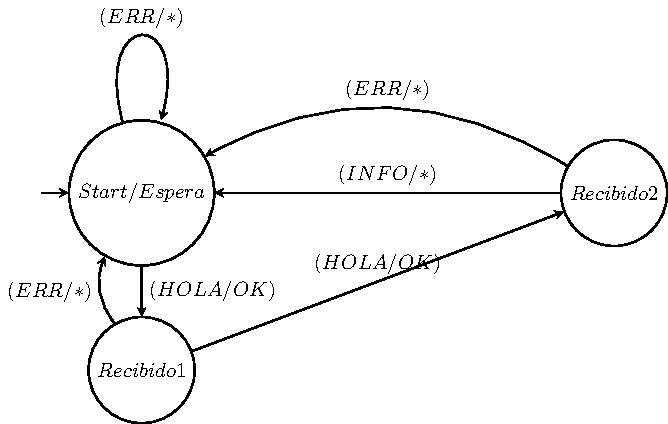
\includegraphics[width=0.8\textwidth]{Diagrama.pdf}
    \caption{Diagrama de estados del servidor.}
\end{figure}
\end{frame}

\begin{frame}
	\frametitle{Diagrama cliente 1}
	\begin{figure}[H]
    \centering
    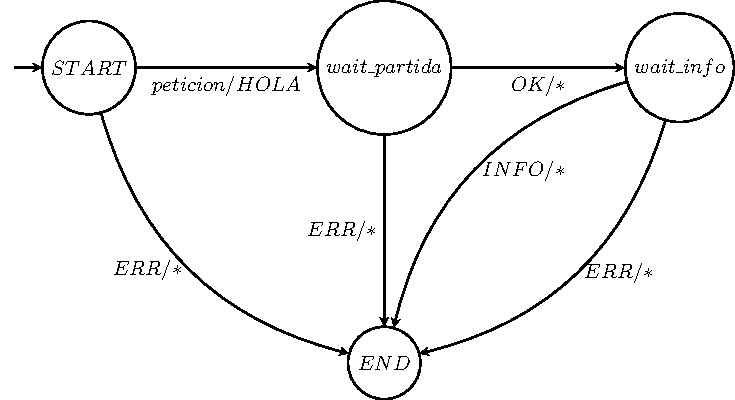
\includegraphics[width=0.8\textwidth]{DiagramaCliente1.pdf}
    \caption{Diagrama de estados del cliente.}
\end{figure}
\end{frame}

\begin{frame}
	\frametitle{Diagrama cliente 2}
	\begin{figure}[H]
    \centering
    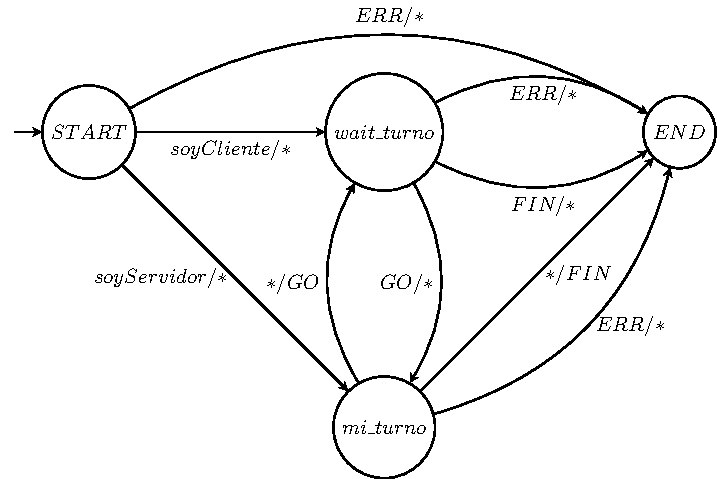
\includegraphics[width=0.8\textwidth]{DiagramaCliente2.pdf}
    \caption{Diagrama de estados del cliente-cliente.}
\end{figure}
\end{frame}


\subsection{Mensajes implicados}
\begin{frame}
	\frametitle{Mensajes}
	\begin{table}[]
\centering

\label{my-label}
\begin{tabular}{lll}
\textbf{Código} & \textbf{Cuerpo} & \textbf{Descripción}                                  \\
000             & ERR             & Error - vuelve al inicio                              \\
001             & OK              & El servidor responde a la petición del cliente.       \\
002             & INFO            & El servidor envia la información de un cliente a otro \\
003             & HOLA            & Recibe la petición por parte del cliente.             \\
004				& GO			  & Acaba el turno, le toca al cliente que recibe		  \\
005				& FIN			  & Fin de partida
\end{tabular}
\caption{Codigo de mensajes}
\end{table}
\end{frame}


\end{document}



